% -*- TeX:de -*-
\NeedsTeXFormat{LaTeX2e}
\documentclass[12pt,a4paper]{article}
\usepackage[german]{babel} % german text
\usepackage[DIV12]{typearea} % size of printable area
\usepackage[T1]{fontenc} % font encoding
%\usepackage[latin1]{inputenc} % most likely on Windows
\usepackage[utf8]{inputenc} % probably on Linux
\usepackage{multicol}

% PLOTTING
\usepackage{pgfplots} 
\usepackage{pgfplotstable}
\usepackage{url}
\usepackage{graphicx} % to include images
\usepackage{tikz}
\usepackage{subfigure} % for creating subfigures
\usepackage{amsmath} % a bunch of symbols
\usepackage{amssymb} % even more symbols
\usepackage{booktabs} % pretty tables
\usepackage{makecell} % multi row table heading

% a floating environment for circuits
\usepackage{float}
\usepackage{caption}

%\newfloat{circuit}{tbph}{circuits}
%\floatname{circuit}{Schaltplan}

% a floating environment for diagrams
%\newfloat{diagram}{tbph}{diagrams}
%\floatname{diagram}{Diagramm}

\selectlanguage{german} % use german

\begin{document}

%%%%%%% DECKBLATT %%%%%%%
\thispagestyle{empty}
			\begin{center}
			\Large{Fakultät für Physik}\\
			\end{center}
\begin{verbatim}


\end{verbatim}
							%Eintrag des Wintersemesters
			\begin{center}
			\textbf{\LARGE WS 2013/14}
			\end{center}
\begin{verbatim}


\end{verbatim}
			\begin{center}
			\textbf{\LARGE{Physikalisches Praktikum\\ für das Bachelorstudium}}
			\end{center}
\begin{verbatim}




\end{verbatim}

			\begin{center}
			\textbf{\LARGE{PROTOKOLL}}
			\end{center}
			
\begin{verbatim}

\end{verbatim}

			\begin{flushleft}
			\textbf{\Large{Experiment (Nr., Titel):}}\\
							%Experiment Nr. und Titel statt den Punkten eintragen
			\LARGE{PW2 - Grundgrößen der Mechanik}	
			\end{flushleft}

\begin{verbatim}

\end{verbatim}	
							%Eintragen des Abgabedatums, oder des Erstelldatums des Protokolls
			\begin{flushleft}
			\textbf{\Large{Datum:}} \Large{23.1.2014}
			\end{flushleft}
			
\begin{verbatim}
\end{verbatim}
							%Namen der Protokollschreiber
		\begin{flushleft}
			\textbf{\Large{Namen:}} \Large{Patrick Braun, Johannes Kurz}
			\end{flushleft}

\begin{verbatim}


\end{verbatim}
							%Kurstag und Gruppennummer, zb. Fr/5
			\begin{flushleft}
			\textbf{\Large{Kurstag/Gruppe:}} \Large{DO/2}
			\end{flushleft}

\begin{verbatim}

\end{verbatim}
							%Name des Betreuers, das Praktikum betreute.
			\begin{flushleft}
			\LARGE{\textbf{Betreuer:}}	\Large{Franz Sachslehner}	
			\end{flushleft}

%%%%%%% DECKBLATT ENDE %%%%%%%
\pagebreak
\setlength{\columnsep}{20pt}
\begin{multicols}{2}

%%%%%%%%%%%%%%%%%%%%%%%%%%%%%%%%%%%%%%%%%%%%%%%%

%\begin{figure}[H]
%	\centering
%	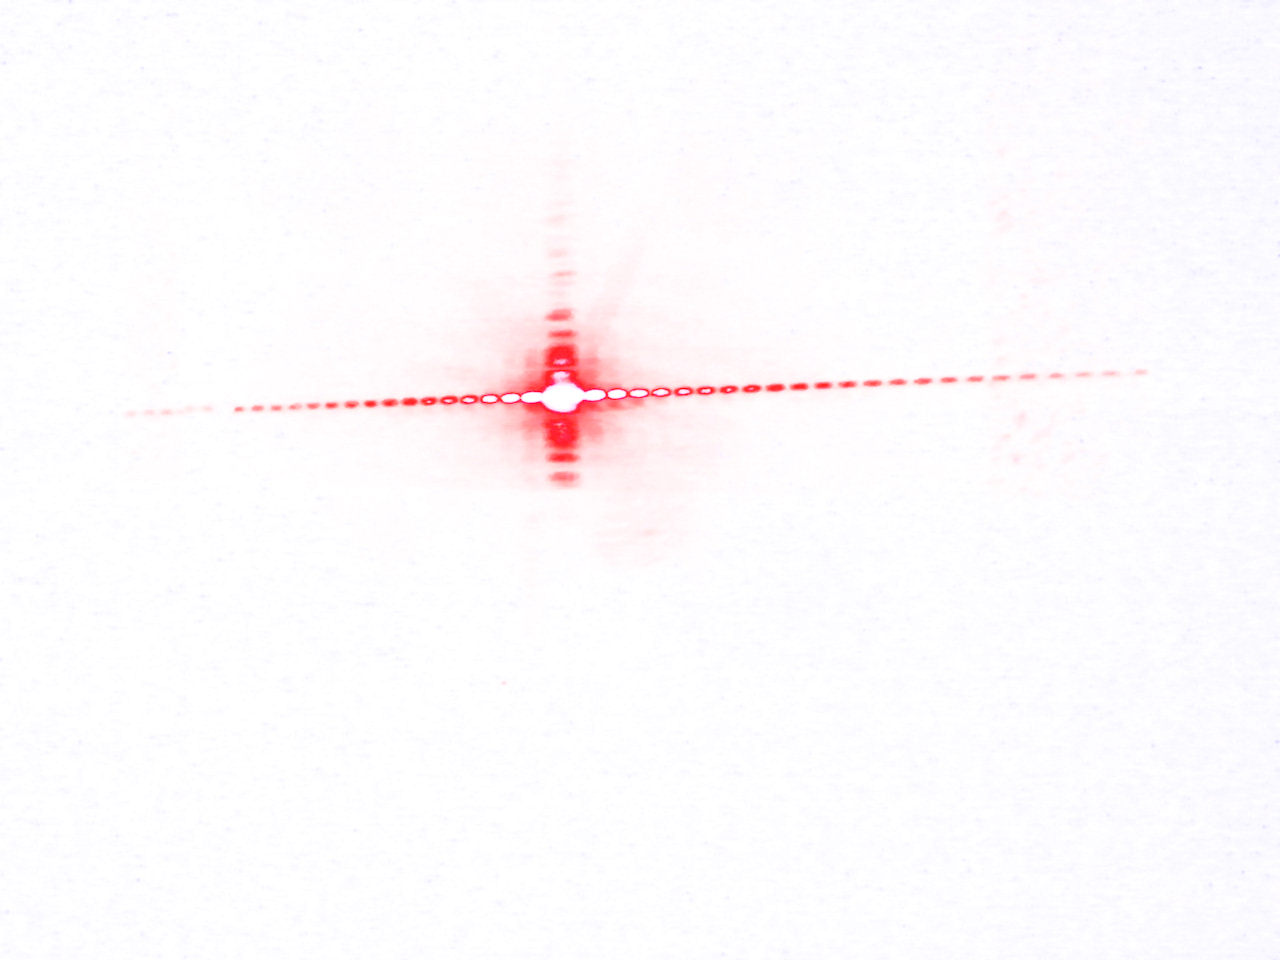
\includegraphics[scale=0.35]{./figure/beugung.png}
%	\caption{Beugungsmuster Einzelspalt (echtes Foto; schwarz durch weiß ersetzt)}
%	\label{fig:beugungsmuster}
%\end{figure}


%\begin{figure}[H]
%	\centering
%	\pgfplotstabletypeset[
%			columns={abstand, n},
%			col sep=&,
%			columns/abstand/.style={precision=2, zerofill, column name=\makecell{$Abstand$\\$(\pm 0.05)[mm]$} }, 
%			columns/n/.style={column name=\makecell{$n$\\$(Ordnung)$}, precision=0},
%			every head row/.style={before row=\hline,after row=\hline\hline},
%			every last row/.style={after row=\hline},
%			every first column/.style={column type/.add={|}{} },
%			every last column/.style={column type/.add={}{|} }
%			]{
%			abstand & n
%			12.9 & 1
%			24.45 & 2
%			37.40 & 3
%			49.35& 4
%			62.45 & 5
%			74.45 & 6
%			87.45 & 7
%			100.25 & 8
%			
%			}
%	\caption{Messwerte Einzelspalt}
%	\label{tab:werte_einzelspalt}
%\end{figure}
%

%%%%%%%%%%%%%%%%%%%%%%%%%%%%%%%%%%%%%%%%
\section{Dichte von Flüssigkeiten}

\subsection{Theorie}

Im ersten Teil von PW2 soll die Dichte einer Flüssigkeit (Kupfersulfat-Lösung) auf 3 verschiedene Arten bestimmt werden, und diese verglichen werden.\\
Die Dichte $\rho$ ist die Masse pro Volumseinheit eines Körpers oder eines Fluids. Im Falle einer homogenen Masseverteilung, wie in diesem Experiment, gilt
$$\rho = \frac{m}{V}$$

Bei gleichem Volumen verhalten sich also die Massen 2er verschiedener Stoffe zueinander genauso, wie deren Dichten.\\
Sind die untersuchten Stoffe keine Festkörper, wirken auf einen in das jeweilige Fluid eingetauchten Senkkörper eine Auftriebskraft. Die Auftriebskräfte verhalten sich ebenso zueinander, wie die Dichten.\\
Hier wird jedoch durch Messung der Masse der verdrängten Flüssigkeit, bei bekanntem Volumen des Senkkörpers, die Dichtemessung durchgeführt.

%Diese beiden Verhältnisse werden benützt um, einmal im Vergleich mit destilliertem Wasser, einmal mit Luft, die Dichte der Testflüssigkeit zu bestimmen.

%$$\rho = \frac{M}{V} = \frac{[kg]}{[m^3]}$$


\subsection{Aufbau und Methoden}
\textbf{Messung mit dem Pyknometer:}\\
Das Pyknometer ist ein Gefäß, um sehr genau bestimmte Volumina eines Fluides einzufüllen. Würden in einem beliebigen Gefäß mit einer größeren Öffnung, die verschiedenen Oberflächenspannungen es zum Ratespiel machen, gleiche Volumina verschiedener Flüssigkeiten einzufüllen, sorgt hier ein genau eingepasster Stöpsel mit Kapillarbohrung dafür, diesen Einfluss praktisch zu eliminieren.\\
Zuerst wird die Masse $m_0$ des leere Gefäßes gemessen, danach das zu messende Fluid eingefüllt. Ist der Verschluss aufgesetzt, muss für eine genaue Messung sämtliche überschüssige Flüssigkeit vom Gefäß und von der Kapillaröffnung beseitigt werden.\\
So werden die Massen von, in guter Näherung gleichen, Volumina von destilliertem Wasser ($m_1$) und der Kupfersulfatlösung ($m_2$) bestimmt.\\
Die Dichte ergibt sich durch:
$$\rho_{Probe}=\frac{m_2-m_0}{m_1-m_0}\cdot \rho_{dest.}$$
Die Dichte des destillierten Wassers $\rho_{dest}$ wird, nach Messung der Raumtemperatur, aus einer Tabelle entnommen.\\
\\
\textbf{Messung mittels Waage:}\\
Auf einer Waage wird ein Galgen montiert, an dem ein Senkkörper angebracht wird ($Volumen=10cm^3$). Dabei ist darauf zu achten, die Waage waagrecht einzurichten, danach wird sie, mit dem Senkkörper frei in der Raumluft hängend, tariert.\\
Anschließend wird ein Gefäß mit der Probeflüssigkeit so unter den Senkkörper gebracht, dass dieser zur Gänze in das Fluid eintaucht. Der Aufbau ist dabei so zu konstruieren, dass die Waage ausschließlich die Gewichtskraft misst, die auf den Senkkörper wirkt, und nicht die des Gefäßes.\\
Die Auftriebskraft auf den Senkkörper wird nun als negatives Gewicht angezeigt. Eigentlich misst die Waage jedoch die Masse der verdrängten Flüssigkeit. Bei bekanntem Volumen des Senkkörpers ergibt sich dadurch die Dichte.\\
\\
\textbf{Digital-Densitometer:}\\
Zuletzt soll die Dichte der Flüssigkeit mit einem Gerät, speziell zur Dichtemessung, bestimmt werden.\\
Dieses gibt direkt eine gemessene Dichte aus.\\
Es ist nur darauf zu achten, die Probenkammer mit der zu messenden Flüssigkeit auszuspülen, um Verunreinigungen zu minimieren.

\subsection{Resultate}

\textbf{Pyknometer:}\\
Leeres Gefäß: $m_0 = (31.4 \pm 0.1)g$\\
mit dest. Wasser: $m_1 = (82.7 \pm 0.1)g$\\
Probeflüssigkeit: $m_2 = (84.6 \pm 0.1)g$\\
\\
Temperatur $T_{dest} = 22.9^\circ \pm 0.1^\circ$\\
$\rho_{dest} = 997.560 \pm 0.025) kg/m^3$
$$\rho_{Probe} = (1034.5 \pm 2.1) kg/m^3$$\\



\noindent \textbf{Auftrieb:}\\

\noindent Volumen des Probekörpers: 10 $cm^3$\\
Verdrängte Flüssigkeit:\\
%dest. Wasser: $m_{Wasser} = (9.973 \pm 0.001)g$\\
%$m_{Probe} = (10.347 \pm 0.001)g$\\
$$\rho_{Probe} = (1034.7 \pm 0.1)kg/m^3$$\\
Nach der Korrektur des Auftriebs durch die Luft:\\
$$\rho_{korrig.} = (1033.5 \pm 0.1)kg/m^3$$\\



\textbf{Densitometer}
%4 Messungen:
%$$\rho_{1.1}:   (1.0347 \pm 0.001) \frac{g}{cm^3}$$
%$$\rho_{1.2}:   (1.0366 \pm 0.001) \frac{g}{cm^3}$$
%Gereinigt:
%$$\rho_{2.1}:   (1.0366 \pm 0.001) \frac{g}{cm^3}$$
$$\rho_{Probe} =   (1036 \pm 1) kg/m^3$$




\subsection{Diskussion}

Die Ergebnisse aus den Messungen mit allen 3 Methoden liegen gut beieinander, für das Pyknometer und die digitale Messung sind sie, innerhalb der Unsicherheit, im gleichen Wertebereich.\\
Lediglich die Auftriebsmessung, nach der Korrektur durch den Auftrieb in Luft, liegt außerhalb des Unsicherheitsbereichs der Digitalmessung:\\

\noindent Pyknom: $\rho_{Probe} = (1034.5 \pm 2.1) kg/m^3$\\
Digital:   $\rho_{Probe}=   (1036 \pm 1) kg/m^3$\\
Auftrieb: $\rho_{Probe} = (1034.7 \pm 0.5)kg/m^3$\\
\\
korrigiert $\rho_{korrig.} = (1033.5 \pm 0.5)kg/m^3$\\
\\
Diese Abweichung kommt auch durch den sehr kleinen Unsicherheitsbereich für die Auftriebsmessung zustande:\\
Da das Volumen des Senkkörpers in der Angabe als bestimmt angenommen wird, und die Konstruktion als fehlerfrei, geht lediglich die Unsicherheit der Waage in das Endergebnis ein.\\
Diese würde lediglich zu einer Unsicherheit von $\pm 0.1 kg/m^3$ führen.\\
Da jedoch auch der Draht, an dem der Senkkörper befestigt ist Flüssigkeit verdrängt, vor allem aber sein Volumen und auch die Konstruktion des Versuchs nicht näher vermessen wurden, wurde ein etwas größerer Unsicherheitsbereich von $\pm 0.5 kg/m^3$ angenommen. Auch dieser ändert, vor allem nach der Korrektur, nichts an der leichten Abweichung.\\
Diese befindet sich aber im Promill-Bereich, und damit durchaus nicht außerhalb der Erwartung für die Ergebnisse aus mehreren Messmethoden bei vorbereiteten Versuchen.\\
Zusätzliche mögliche Ursachen sind Verunreinigungen am Senkkörper, in der Flüssigkeit sowie Fehler beim waagrechten Ausrichten der Waage.\\
\\
Die Methode mit dem Pyknometer benützt 4 Messgrößen (die 3 Massen und die Raumtemperatur) und hat daher die größte Unsicherheit der 3 Methoden.\\
\\
Das sehr einfach anzuwendende Digital-Densitometer liefert, nach 2 Ausspülversuchen, innerhalb der Messunsicherheit, einheitliche Ergebnisse (es wurden nach den ersten beiden Messungen zur Spülung, 2 weitere durchgeführt, beide mit dem gleichen Ergebnis).\\
\\
\textbf{Aufgabe 5: Dichtemessung von Festkörpern}\\
Für die Dichtebestimmung der vorgeschlagenen kleinen Glaskügelchen (klein genug um in das Densitometer zu passen) wäre ein Ansatz, diese in einer Flüssigkeit mit bekannter Dichte, also als eine Art Lösung, zu verwenden.\\
Wir sind jedoch nicht sicher, ob dann, für die Waage und das Densitometer die gleiche Messmethode, inklusive Korrektur der verwendeten Flüssigkeit geeignet sind. Dazu wäre auch das Verhältnis beider Stoffe nötig. Mit der Waage könnte das Masseverhältnis leicht bestimmt werden, eine reine Densitometer-Dichtebestimmung scheint fraglich.\\
Um diese Frage vollständig zu beantworten, müssten wir noch einmal an den Messgeräten experimentieren.

%Densiometer.. 4 Messungen.. erste nicht so toll

%%%%%%%%%%%%%%%%%%%%%%%%%%%%%%%%%%%%%%%%
\section{Bewegungen, Kräfte und Stöße am Luftkissentisch}

\subsection{Theorie, Aufbau und Methoden:}
In den Versuchen 2 - 5 von PW2 sollen einfache Bewegungen und Stöße 2er Körper am Luftkissentisch herbeigeführt, aufgezeichnet und untersucht werden.\\
Dabei soll der grafische wie numerische Umgang mit Vektoren geübt werden, und die Erhaltungssätze für Impuls und Energie überprüft bzw. dargestellt werden.\\
\\
Dazu werden Gleiter verwendet, die sich auf einem Luftkissen bewegen, um als praktisch reibungsfrei idealisiert werden zu können. Diese bewegen sich auf einem Metallpapier, auf dem ein Stift am Gleiter 50 mal pro Sekunde einen kurzen Strich zeichnet. Aus diesen Spuren lassen sich die Bahnen der Gleiter, sowie ihre Bewegung mit der Zeit darstellen.\\
5 Striche entsprechen also dem Weg des Stiftes in 0.1s.\\
\\
Als erste wird eine \textbf{gleichmäßig beschleunigte Bewegung} dargestellt.\\
Die Kraft, von der diese Beschleunigung ausgeht, ist die Gravitationskraft.\\
Dazu wird ein Gewicht (Masse $m$) durch einen Faden mit dem Gleiter (Masse $M$) verbunden, das, über ein Rad am Rand des Tisches gelagert, fallen kann, und somit den Gleiter zieht:\\
$$F=m \cdot g = (m+M)a + (Mg \mu_g )$$
Die vom fallenden Gewicht erzeugte Kraft beschleunigt die gesamte Masse mit der zu bestimmenden Beschleunigung $a$, und muss dabei die Reibung des Gleiters (Gleitreibungskoeffizient $\mu_g$) überwinden.\\
Aus den Ortsvektoren zu jeder 10tel Sekunde kann ein Bewegungsdiagramm gezeichnet werden, das näherungsweise einem Polynom 2. Ordnung entspricht. Durch differenzieren erhält man die Geschwindigkeit des Gleiters $v(t)$ und seine Beschleunigung $a(t)$.\\
\\
Zweitens wird eine \textbf{kräftefreie Bewegung} dargestellt. Der Gleiter bewegt sich in Rotation und Translation über das Papier, wobei der Stift im Zentrum wie gehabt die Bewegung des gesamten Körpers aufzeichnet, während ein zweiter Stift am Rand angebracht wird, um die Rotation darzustellen.\\
Indem gleichzeitig zu Papier gebrachte Markierungen miteinander verknüpft werden, lässt sich die Drehung mit der Fahrt des Gleiters in Beziehung setzen.\\
Die Geschwindigkeit des Außenstiftes kann als Superposition aus Schwerpunktsbewegung und Rotation dargestellt werden:
$$\vec v = \vec v_s + \vec \omega \times \vec r$$
\\
Die dritte Bewegung, die aufgezeichnet wird, ist ein \textbf{elastischer Stoß}.\\
Dazu wird ein zweiter Gleiter auf den Tisch gebracht und beide werden mit Federringen ausgestattet, um sich gegenseitig abzustoßen. Einer der beiden Gleiter wird zudem mit einem Zusatzgewicht von etwa 1/2kg beschwert.\\
Theoretisch gelten in diesem Fall 3 Erhaltungssätze:\\
- Impulserhaltung\\
- Schwerpunktsatz\\
- Energieerhaltung.\\
\\
Alle 3 sollen gezeigt und überprüft werden, indem gleichzeitig aufgezeichnete Striche beider Gleiter in Beziehung gesetzt werden. So kann die Bewegung des Schwerpunkts dargestellt werden.\\
Durch die Geschwindigkeitsvektoren vor und nach dem Stoß (eine bestimmte Länge zu einer definierten Zeit), lässt sich die Impulserhaltung grafisch, also auch numerisch überprüfen. Dazu werden die Vektoren (skaliert um die Masse) vor dem Stoß, sowie diejenigen nach dem Stoß addiert (entweder in Zahlen, oder durch hintereinander-zeichnen).\\
Treffen sich die Spitzen der Impulsvektorsummen, wäre also die Erhaltung gezeigt.\\
\\
Zuletzt soll noch ein \textbf{inelastischer Stoß} untersucht werden.\\
Dazu werden die Gleiter, statt mit Federringen, nun mit Ringen aus Klettverschluss ausgerüstet, um nach dem Stoß aneinander zu haften und eine gemeinsame Bahn zu beschreiben.\\
In diesem Versuch wird nur der schwerere Gleiter $M_1$ in Bewegung versetzt, der leichtere $M_2$ befindet sich zunächst in Ruhe und wird vom schwereren angestoßen.\\
Da nun ein Teil der Energie der beiden Gleiter beim Stoß in Verformung und Wärme umgewandelt wird, ergibt sich diese innere Energie $U$ durch die Differenz der kinetischen Energien vor und nach dem Stoß:
$$U=\frac{M_1 \vec v_1^2}{2}-\frac{(M_1+M_2) \vec v'^2}{2}$$



%g \ldots Gravitationsbeschleunigung Erde\\
%m \ldots kleine Masse am Faden\\
%M \ldots große Masse am Tisch\\
%$\mu$ \ldots Reibungskoeffizient von M\\
%a \ldots Beschleunigung beider Massen\\
%
%$$F_g = m * g = [N]$$
%$$F_{Reibung} = M*g*\mu$$
%$$F_{mM} = (m+M)*a$$
%$$F_{g} = F_{mM} + F_{Reibung}$$
%$$m * g = M*g*\mu + (m+M)*a$$

\end{multicols}

\subsection{Resultate}



%%%% Beschleunigte und Kraeftefreie Bewegung
%\pagebreak
%\end{multicols}

\begin{figure}[H]
	\centering
	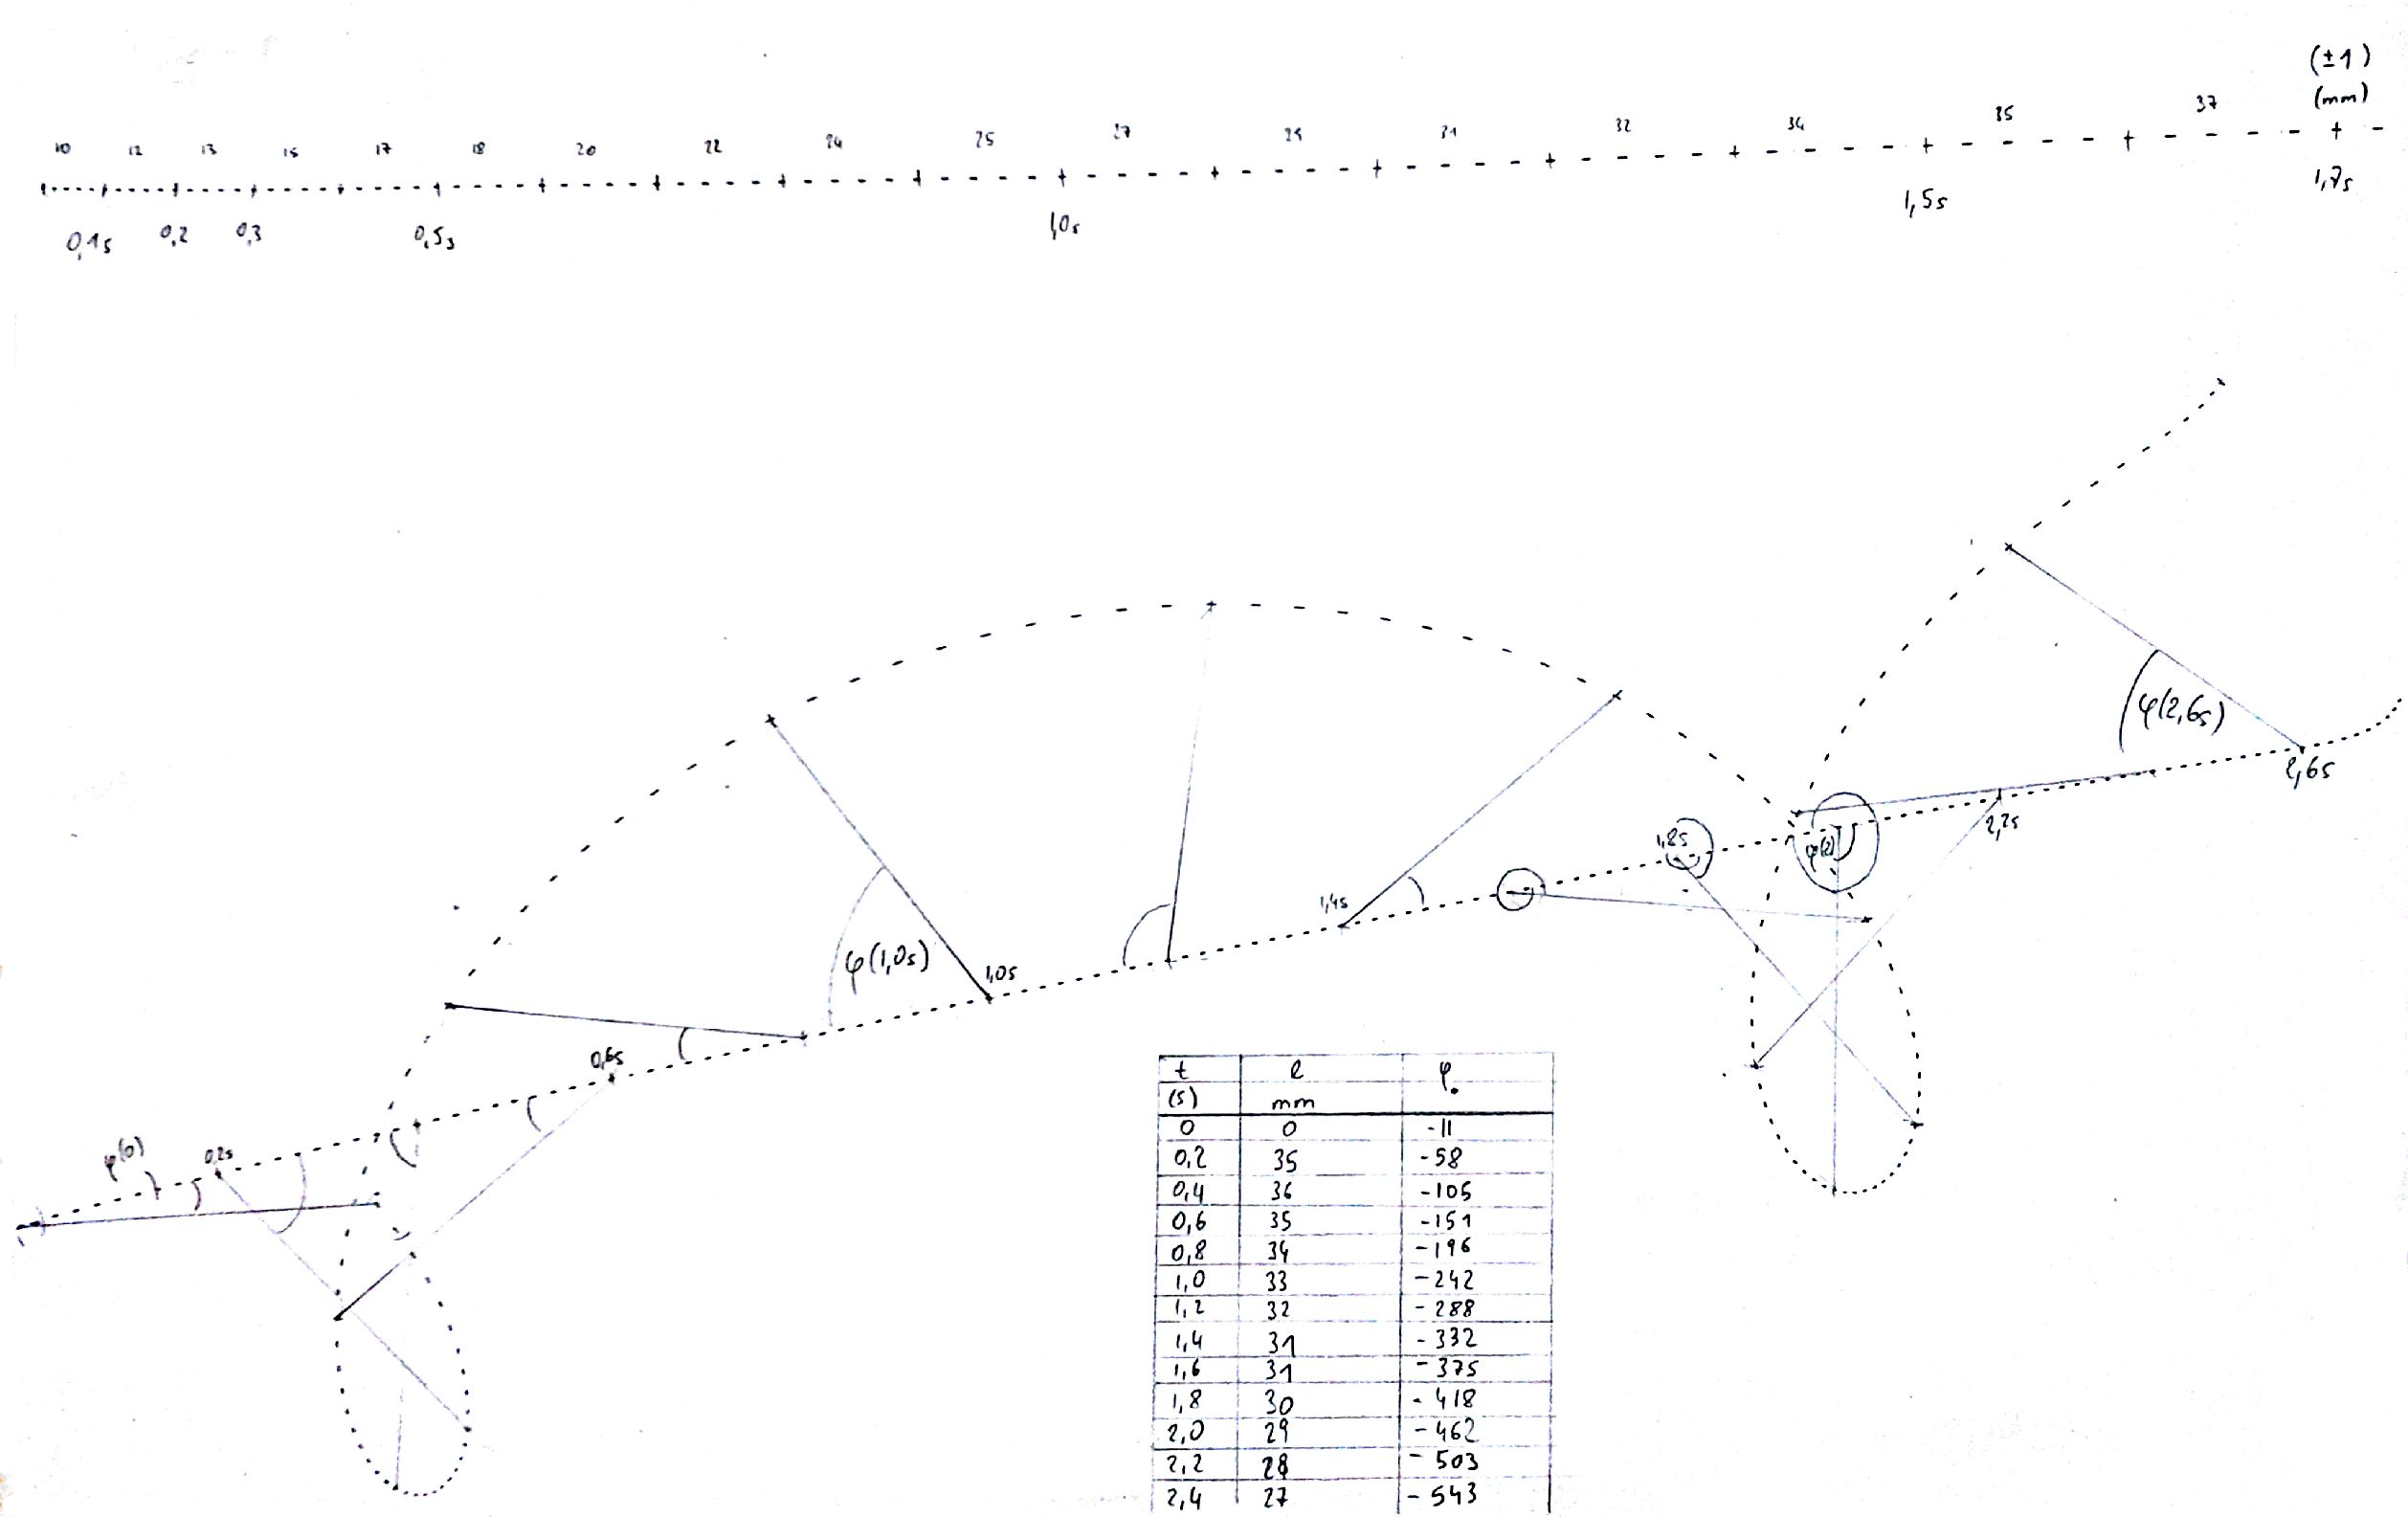
\includegraphics[scale=0.25, angle=-90]{./figure/bewegungen.jpg}
	\caption{Eindimensionale Beschleunigung und kräftefreie Bewegung}
	\label{fig:bewegungen}
\end{figure}



\begin{figure}[H]
	\centering
	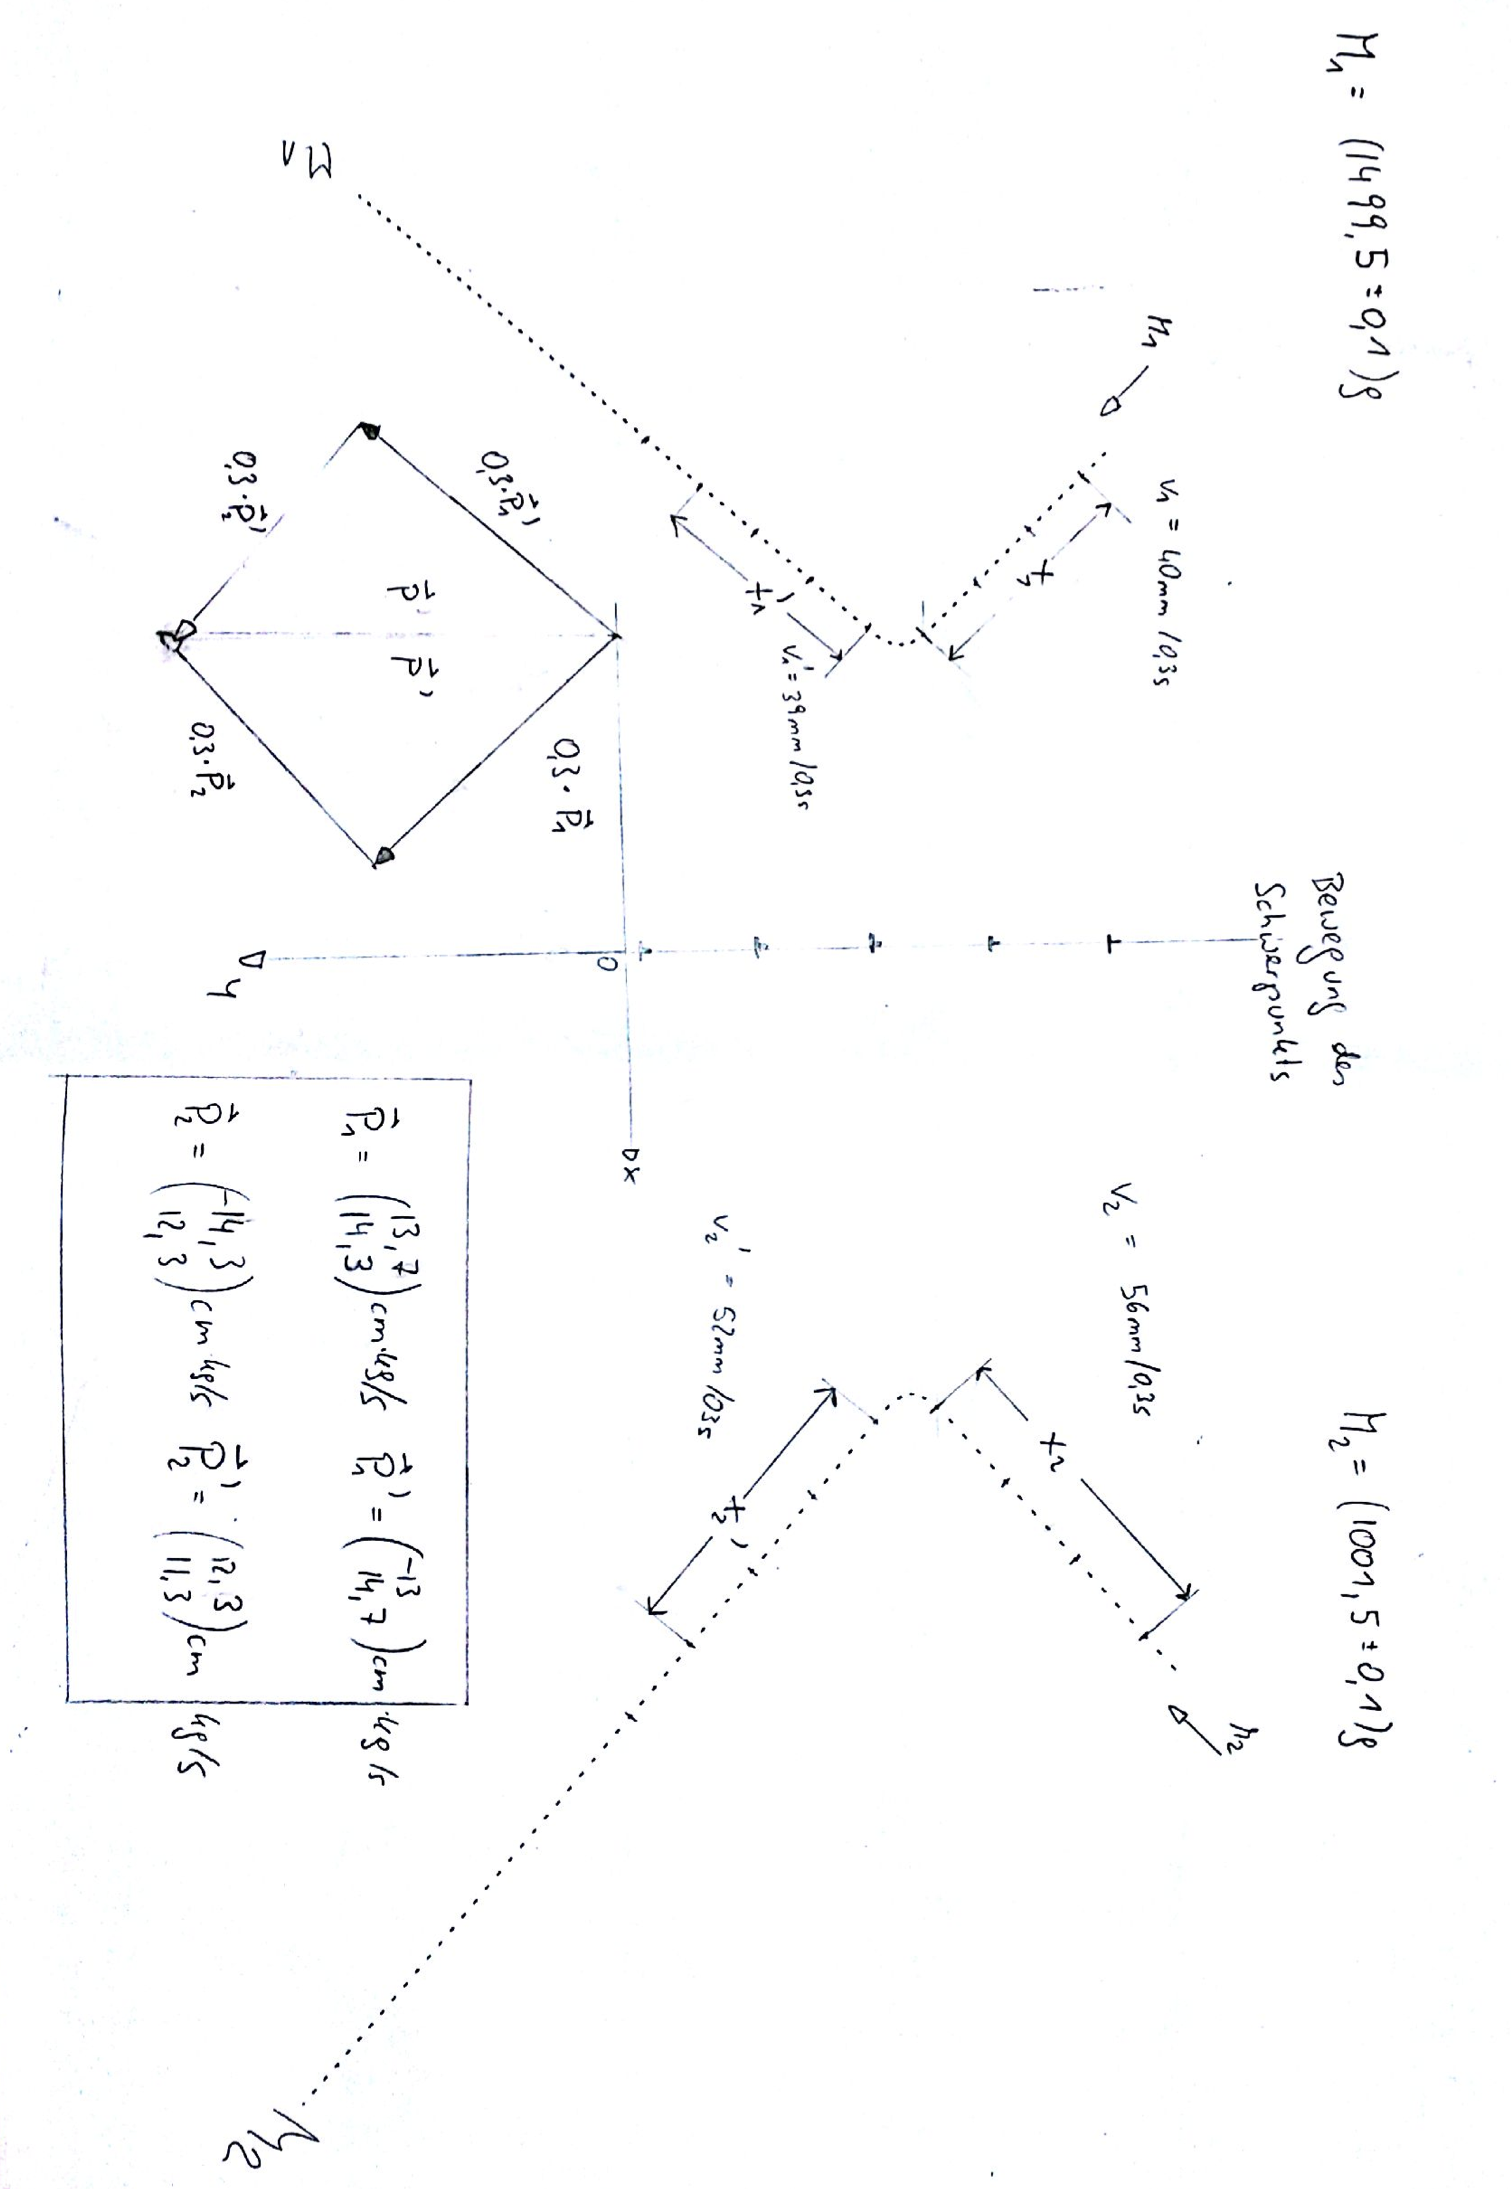
\includegraphics[scale=0.9]{./figure/elastischer_stoss.png}
	\caption{Elastischer Stoß, Schwerpunktsbewegung und Impulserhaltung}
	\label{fig:elastisch_stoss}
\end{figure}

\begin{figure}[H]
	\centering
	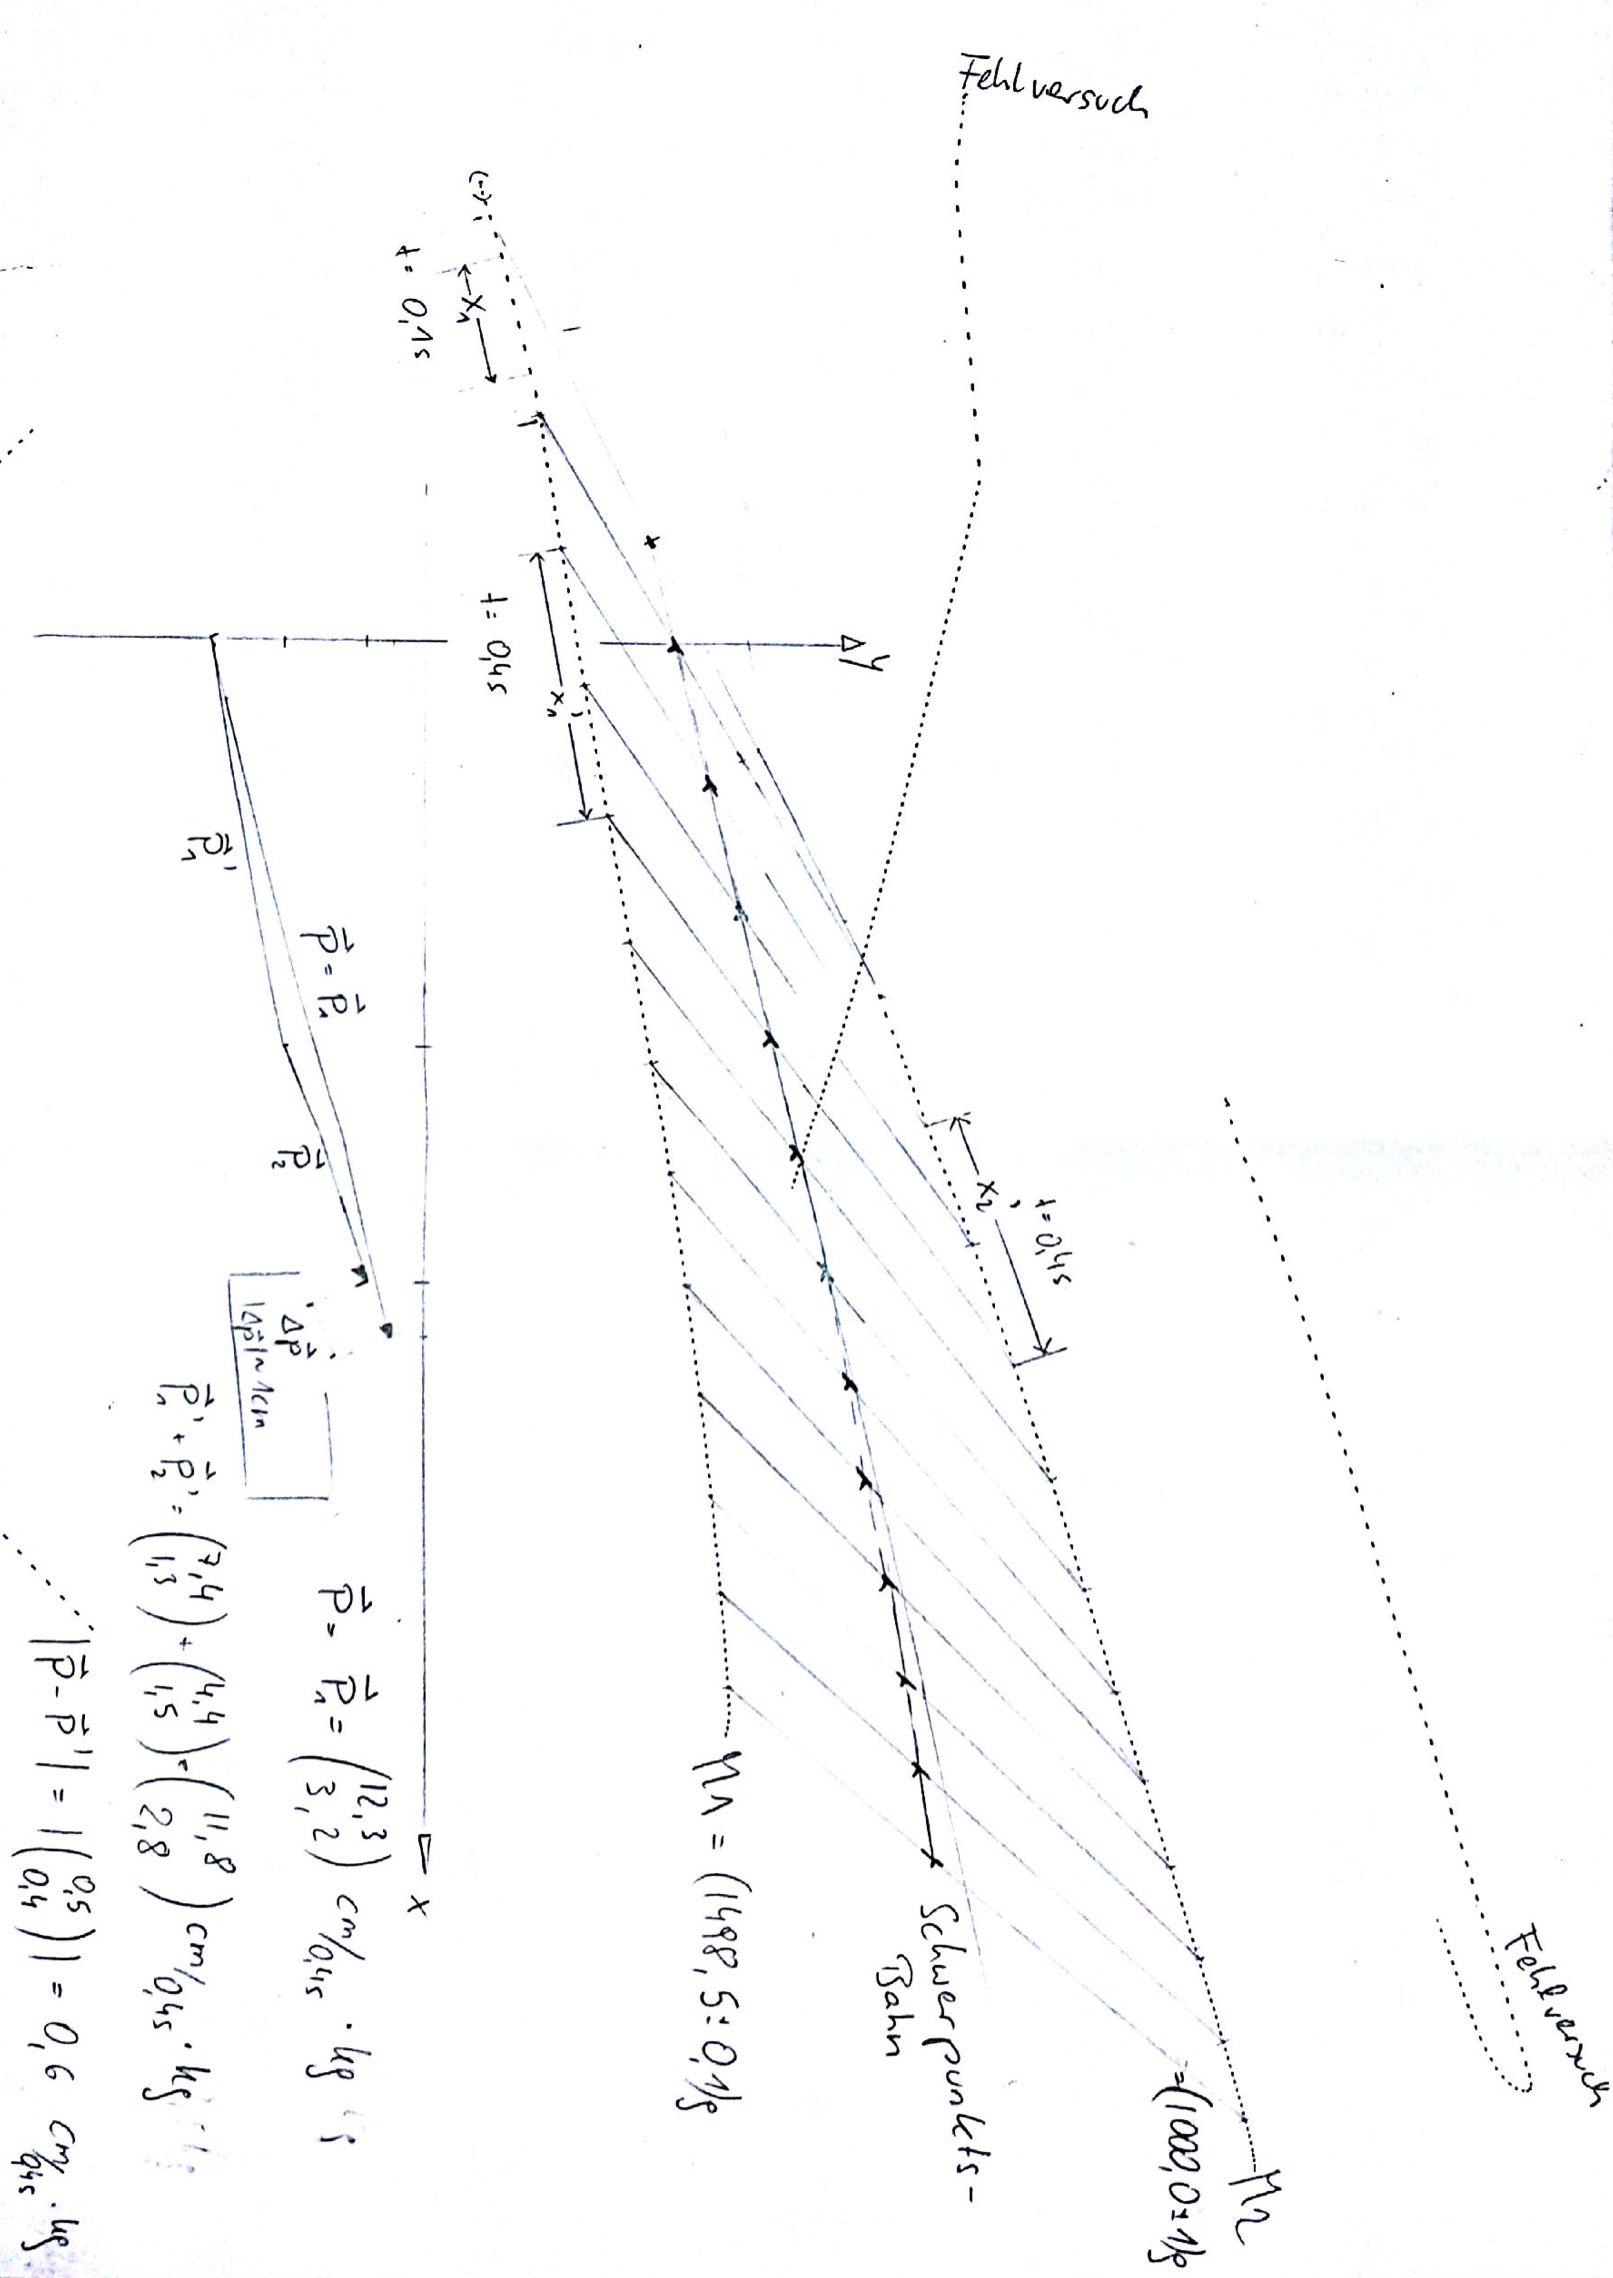
\includegraphics[scale=0.75]{./figure/inelastischer_stoss.png}
	\caption{Unelastischer Stoß, Schwerpunktsbewegung und Impulserhaltung}
	\label{fig:inelastisch_stoss}
\end{figure}





%\begin{multicols}{2}


\begin{figure}[H]
	\centering
	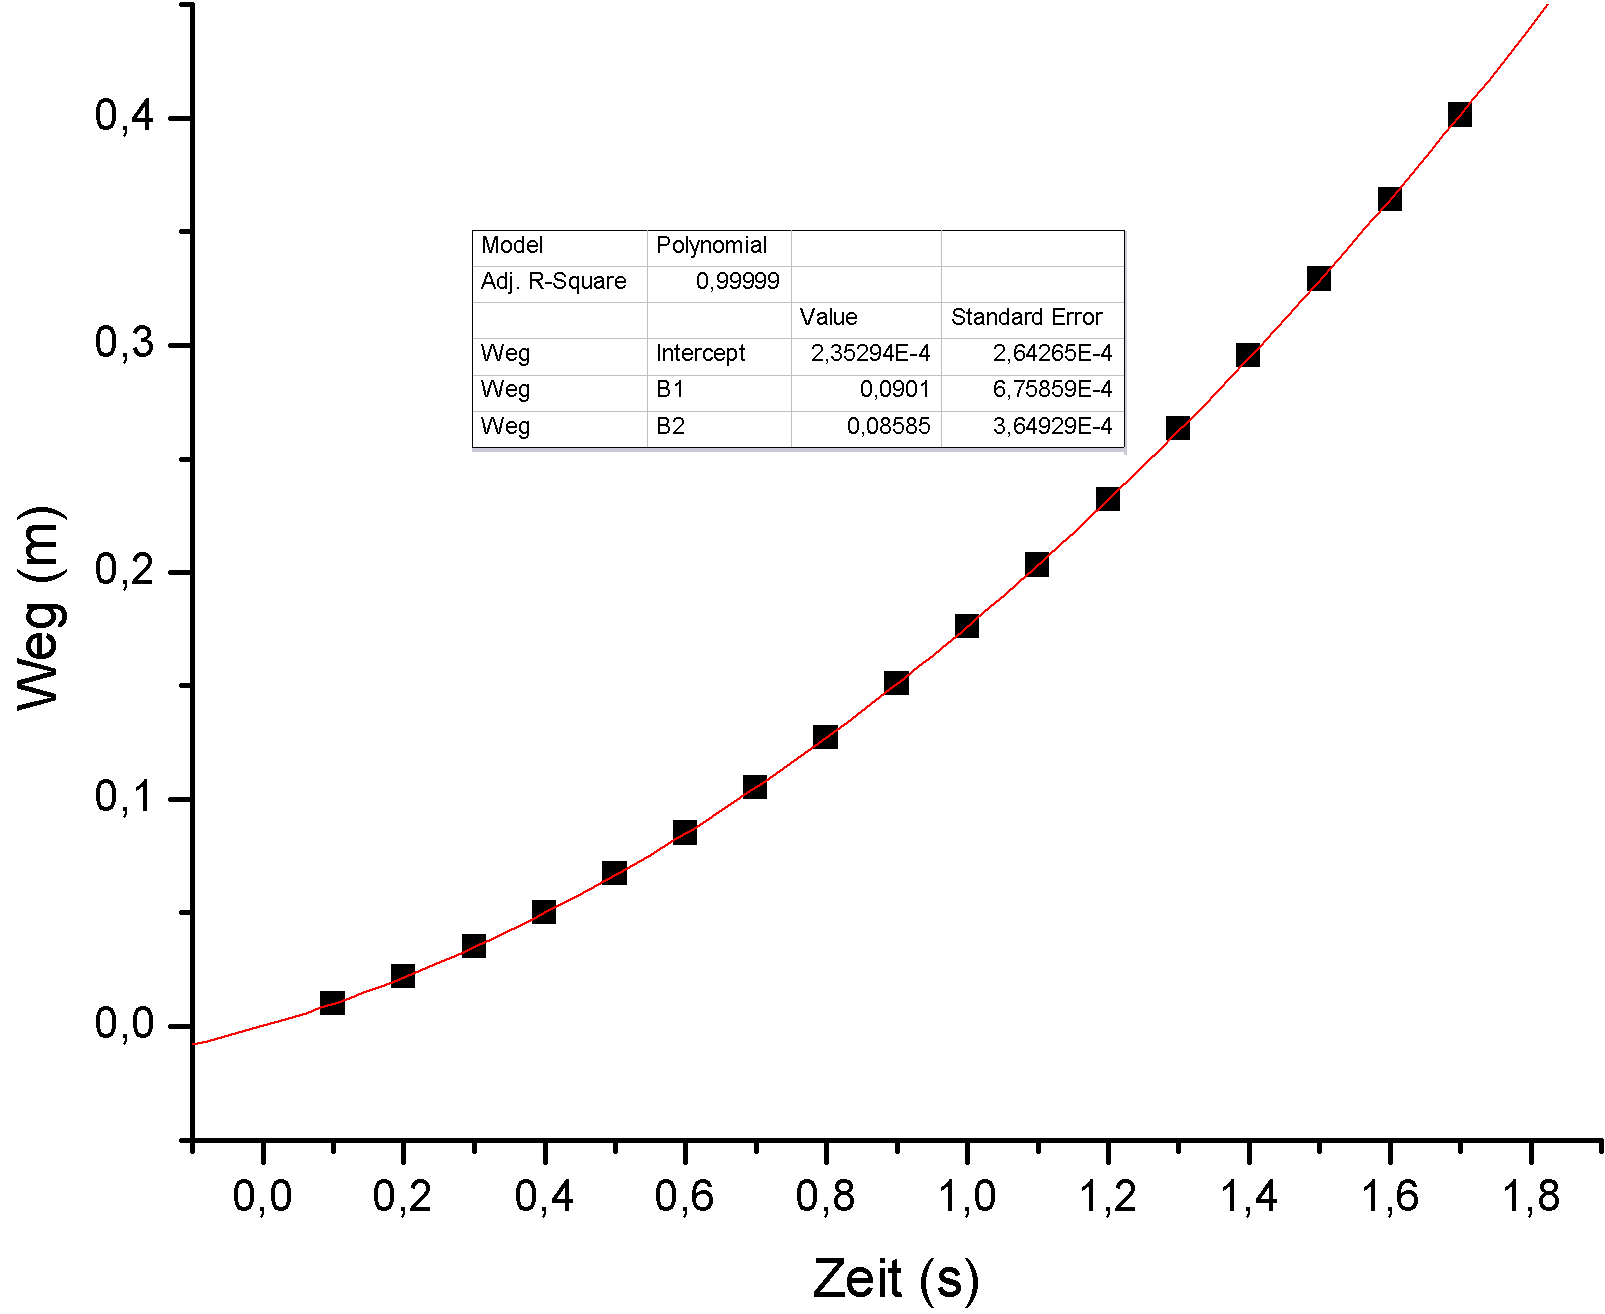
\includegraphics[scale=0.53]{./figure/x_t_diagram.png}
	\caption{x(t)-Diagramm der gleichmäßig beschleunigten Bewegung}
	\label{fig:lin_bewegung}
\end{figure}
\begin{figure}[H]
	\centering
	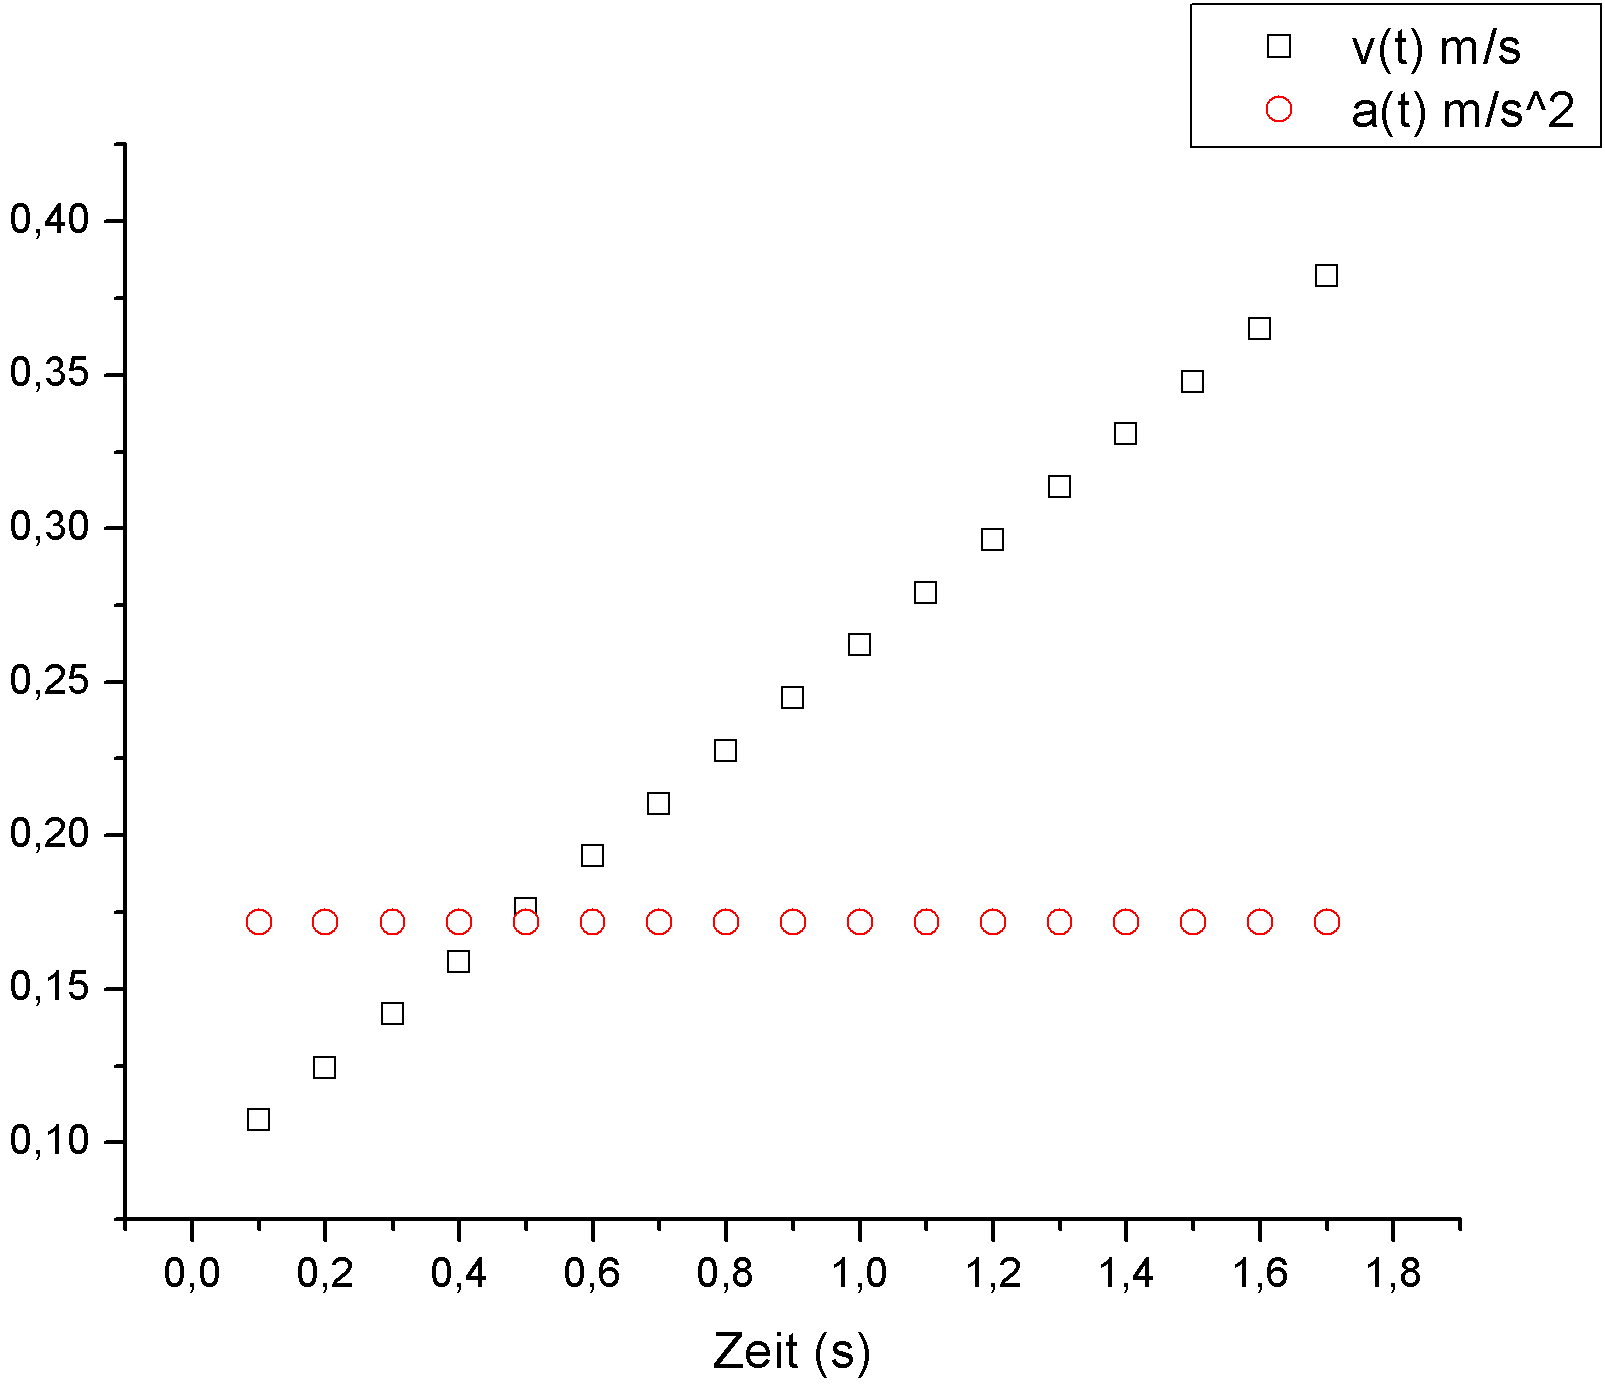
\includegraphics[scale=0.27]{./figure/v_a_t_diagram.png}
	\caption{v(t)- und a(t)-Diagramm der gleichmäßig beschleunigten Bewegung}
	\label{fig:lin_bewegung_v_a}
\end{figure}



\begin{multicols}{2}

\noindent \textbf{Gleichmäßig beschleunigte Bewegung:}\\

In Abb. \ref{fig:lin_bewegung} ist die Ortsentwicklung des Gleiters nach der Zeit zu sehen.
Der Polynomiale Fit (2. Ordnung) ergibt als Bewegungsgleichung:
$$x(t)=x_0 + v_0 \cdot t + a \cdot \frac{t^2}{2}$$

$$x_0=(0.000 \pm 0.024)cm$$
$$v_0=(9.010 \pm 0.068)cm/s \cdot $$
$$a=( 8.585 \pm 0.037) cm/s^2 $$

Die Kraft, die auf das System wirkt, falls M reibungsfrei gleitet, ist:
$$F= (0.08727 \pm 0.00038) N$$

Der Gleitreibungskoeffizient $\mu_g$ ist:
$$\mu_g = (0.010736 \pm 0.00092)$$
(es wird $g=9.81m/s^2$ angenommen)\\
\\
\\


\noindent \textbf{Kräftefreie Bewegung:}\\
Siehe Abb. \ref{fig:lin_bewegung}\\

%%%% Grafik x(t),v(t),a(t) der kräftefreien bewegung

%%%% Grafik $\phi (t)







\noindent \textbf{Elastischer Stoß:}\\

siehe Abb. \ref{fig:elastisch_stoss}

\noindent Geschwindigkeiten:\\
vor dem Stoß:\\
$\vec v_1 =\binom{9.2}{9.5} cm/s$\\
$\vec v_2 =\binom{-14.3}{12.3} cm/s$\\
\\
nach dem Stoß:\\
$\vec v_1' =\binom{-8.7}{9.8} cm/s$\\
$\vec v_2 '=\binom{12.3}{11.3} cm/s$\\
\\
\\
Impulse:\\
vor dem Stoß:\\
$\vec p_1 =\binom{13.7}{14.3} kg\cdot cm/s$\\
$\vec p_2 =\binom{-14.3}{12.3} kg\cdot cm/s$\\
\\
nach dem Stoß:\\
$\vec p_1' =\binom{-14.3}{12.3} kg\cdot cm/s$\\
$\vec p_2 '=\binom{12.3}{11.3} kg\cdot cm/s$\\
\\
\\
Impulserhaltung:\\
$\vec p_1 + \vec p_2 = \binom{-0.6}{26.6} kg\cdot cm/s$\\
$\vec p_1' + \vec p_2' = \binom{-0.7}{26.0} kg\cdot cm/s$\\
$\Delta \vec p =  \binom{0.1}{0.6} kg\cdot cm/s$\\
\\
\\
kinetische Energie:\\
vor dem Stoß:\\
$T = (0.030 \pm 0.003) J$\\
nach dem Stoß:\\
$T'=(0.027 \pm 0.003) J$\\
\\
\\
Der Schwerpunkt beschreibt in guter Näherung eine Gerade.\\
\\
\textbf{Inelastischer Stoß:}\\
siehe Abb. \ref{fig:inelastisch_stoss}

Geschwindigkeiten:\\
vor dem Stoß:\\
$\vec v_1 =\binom{21.0}{5.0} cm/s$\\
$\vec v_2 =\binom{0}{0} cm/s$\\
\\
nach dem Stoß:\\
$\vec v_1' =\binom{11.0}{2.0} cm/s$\\
$\vec v_2 '=\binom{11.0}{3.8} cm/s$\\
\\
\\
Impulse:\\
vor dem Stoß:\\
$\vec p_1 =\binom{12.3}{3.2} kg\cdot cm/s$\\
$\vec p_2 =\binom{0}{0} kg\cdot cm/s$\\
\\
nach dem Stoß:\\
$\vec p_1' =\binom{7.4}{1.3} kg\cdot cm/s$\\
$\vec p_2 '=\binom{4.4}{1.5} kg\cdot cm/s$\\
\\
\\
Impulserhaltung:\\
$\vec p_1 + \vec p_2 = \binom{12.3}{3.2} kg\cdot cm/s$\\
$\vec p_1' + \vec p_2' = \binom{11.8}{2.8} kg\cdot cm/s$\\
$\Delta \vec p =  \binom{0.5}{0.4} kg\cdot cm/s$\\
\\
\\
\\
\\
kinetische Energie:\\
vor dem Stoß:\\
$T = (0.035 \pm 0.003) J$\\
nach dem Stoß:\\
$T'=(0.027 \pm 0.003) J$\\
\\
$\Delta T= (0.008 \pm 0.004) J$
\\
\\


\subsection{Diskussion}
\textbf{Gleichförmig beschleunigte Bewegung:}\\
Der Polynom-Fit 2. Ordnung in Abb. \ref{fig:lin_bewegung} sitzt gut auf den Datenpunkten der Ortsvektoren. Wie erwartet verläuft die gleichmäßig beschleunigte Bewegung also in der Form einer Parabel.\\
Die Bewegungsgleichung gibt also auch, durch Differentiation, einen linearen Geschwindigkeitsanstieg und eine konstante Beschleunigung (Abb. \ref{fig:lin_bewegung_v_a}).\\
Auch der Gleitreibungskoeffizient $\mu_g$ ist, wie erwartet sehr klein. Reibung wird jedoch nicht nur vom Gleiter auf dem Luftpolster erzeugt, ein kleiner Anteil entsteht auch durch das Rad, über das der Faden läuft.\\
\\
\textbf{Kräftefreie Bewegung:}\\
Der Schwerpunkt des Gleiters bewegt sich fast auf einer Geraden, und ist dabei fast unbeschleunigt.\\
In erster Näherung entsteht die erwartete gerade Bewegung mit konstanter Geschwindigkeit. Einleichter Reibungsverlust sowie eine Ablenkung durch Assymetrien in der Masseverteilung lassen sich jedoch nicht ganz beseitigen.\\
Obwohl die Geschwindigkeit als konstant angenommen werden kann, wurde ein Polynom-Fit 2. Ordnung durchgeführt. Dieser gibt die leichte Bremsung von etwa $1cm/s^2$.\\
\\
Ähnliches gilt für die Winkelgeschwindigkeit, die in erster Näherung konstant ist, jedoch leicht abnimmt mit der Zeit.\\
Die aufgezeichnete Bewegung wäre bei mehreren Versuchen und einer längeren Bahn sicherlich noch verbesserungswürdig, es genügt jedenfalls um die theoretischen Beziehungen gut zu veranschaulichen, sodass sich ein ökonomischer Mehraufwand im Rahmen des Praktikums wohl nicht lohnen würde.\\
\\
\textbf{Elastischer Stoß:}\\
Sowohl graphisch (Abb. \ref{fig:elastisch_stoss}), als auch numerisch, ist die Impulserhaltung näherungsweise gezeigt. Die in den beiden anderen Versuchen gefundenen Verluste greifen sicherlich auch hier leicht ein.\\
Auch die kinetischen Energien vor und nach dem Stoß sind, mit einer etwas großzügigen Unsicherheitsabschätzung, bedingt durch die Methode der Vermessung ohne geeigneten technischen Zeichentisch, gleich im geforderten Bereich.\\
Zusätzlich zu den Reibungsverlusten (diesmal von 2 Gleitern) sind sicherlich auch geringe Energieverluste beim Stoß nicht zu verhindern, da reale Stöße weder völlig elastisch, noch inelastisch sind.\\
\\
\textbf{Inelastischer Stoß:}\\
Etwas ungenauer als beim elastischen Stoß, ist auch hier die Impulserhaltung näherungsweise gezeigt. Zusätzlich zu den bereits besprochenen Verlusten, ist festzustellen, dass dieses Experiment nicht besonders gut geglückt ist.\\
Der Weg vor dem Stoß ist sehr kurz geraten und die Gleiter sind mittiger, als gewünscht, aufeinandergetroffen (Abb. \ref{fig:inelastisch_stoss}).\\
Es sind also durchaus große Unsicherheiten in der graphischen Vermessung zu erwarten.\\
\\
Der Schwerpunkt führt zuerst eine gerade Bewegung durch und bekommt gegen Ende einen leichten Drift. Das könnte aufgrund verschiedener Reibungen beider Gleiter entstehen.\\
\\
Die Differenz der kinetischen Energien, vor und nach dem Stoß, ist, im Gegensatz zum elastischen Stoß, hier eindeutig und liegt etwa bei 10-20\% der ursprünglichen Energie (wieder wurde die Unsicherheit aus den erwähnten Gründen groß abgeschätzt).


%%%%%%%%%%%%%%%%%%%%%%%%%%%%%%%%%%%%%%%%


\section{Quellen}
$[1]$ Anleitung, \url{http://www.univie.ac.at/anfpra/neu1/pw/pw2/PW2.pdf}\\
\end{multicols}

\end{document}